\RequirePackage[l2tabu,orthodox]{nag}
\documentclass{article}
\usepackage{amsthm}
\usepackage{amssymb}
\usepackage{mathtools}
\usepackage{minted}

\usepackage[colorlinks=true,pagebackref,hyperindex,citecolor=myblue,linkcolor=mygreen,urlcolor=mygreen]{hyperref}
\usepackage[top=1in, bottom=1in, left=1.25in, right=1.25in]{geometry}

\usepackage{amsmath}
\usepackage{amsfonts}
\usepackage{amssymb}

\usepackage{color}
\usepackage[dvipsnames]{xcolor}
%\definecolor{myblue}{rgb}{0.16, 0.32, 0.75}
\definecolor{myblue}{rgb}{0.0, 0.45, 0.73}
\definecolor{mygreen}{rgb}{0.05, 0.5, 0.06}

\usepackage{mathrsfs}
\usepackage[mathcal]{euscript}
\usepackage{mathtools}

\usepackage{enumitem}

\usepackage{float}
\usepackage[center]{caption}

%\usepackage{setspace}
%\singlespacing
%\onehalfspacing
%\doublespacing
%\setstretch{1.1}
\parskip 0.1cm


%%%%%%%%%%%%%%%%%% Clever Ref %%%%%%%%%%%%%%%%%%
\usepackage{cleveref}
\crefname{equation}{Eq.}{Eqs.}
\crefname{theorem}{Theorem}{Theorems}
\crefname{lemma}{Lemma}{Lemmata}
\crefname{corollary}{Corollary}{Corollaries}
\crefname{proposition}{Proposition}{Propositions}
\crefname{definition}{Definition}{Definitions}
\crefname{rem}{Remark}{Remarks}
\crefname{example}{Example}{Examples}
\crefname{conventions}{Conventions}{Conventions}
\crefname{setup}{Setup}{Setup}
\crefname{question}{Question}{Question}
\crefname{figure}{Figure}{Figures}


%THEOREM ENVIRONMENTS
\newtheorem{theorem}{Theorem}[section]
\newtheorem{lemma}[theorem]{Lemma}
\newtheorem{corollary}[theorem]{Corollary}
\newtheorem{proposition}[theorem]{Proposition}

\newtheorem*{nak*}{Nakayama's Lemma}


%DEFINITION STYLE ENVIRONMENTS
\theoremstyle{definition}
\newtheorem{definition}[theorem]{Definition}
\newtheorem{definition-theorem}[theorem]{Definition/Theorem}
\newtheorem{setup}[theorem]{Setup}
\newtheorem{notation}[theorem]{Notation}
\newtheorem{conventions}[theorem]{Conventions}
\newtheorem{example}[theorem]{Example}

%REMARK STYLE ENVIRONMENTS 
\theoremstyle{remark}
\newtheorem{remark}[theorem]{Remark}
\newtheorem{convention}{Convention}

\numberwithin{equation}{section} %Can replace {subsection} with {theorem} if you want
\numberwithin{figure}{theorem} %Can replace {subsection} with {theorem} if you want

%%%%%%%%

%\newcommand{\pagebreak}{\newpage}
\renewcommand{\pagebreak}{ }


\mathchardef\ordinarycolon\mathcode`\:
\mathcode`\:=\string"8000
\begingroup \catcode`\:=\active
  \gdef:{\mathrel{\mathop\ordinarycolon}}
\endgroup

%%%%%%%%%%%%%%%%%% To-Do %%%%%%%%%%%%%%%%%%
\usepackage[textwidth=2.5 cm,textsize=small,shadow,
%disable
%%option disable removes the notes
]{todonotes}
\newcommand{\drew}[2][]
{\todo[linecolor=green,backgroundcolor=green!10,caption={}, #1]{#2}}
\newcommand{\emily}[2][]
{\todo[linecolor=gray,backgroundcolor=gray!20,caption={}, #1]{#2}}
\newcommand{\perry}[2][]
{\todo[linecolor=blue,backgroundcolor=blue!20,caption={}, #1]{#2}}


\begin{document}
\title{ 
Formalizing Commutative Algebra in Coq: \\
Nakayama's Lemma\thanks{Source code for this work is available on the following
site: \url{https://github.com/ku-sldg/algebra}}
}

\date{}

\author{ 
	Andrew Cousino \\ {\ttfamily acousino@ku.edu}
	\and 
	Emily E.\ Witt\thanks{Witt acknowledges support from NSF CAREER Award
    DMS-1945611 and the 2022-23 Ruth I.\, Michler Memorial Prize from the
    Association for Women in Mathematics.} \\ {\ttfamily witt@ku.edu}
  \and 
	Perry Alexander \\ {\ttfamily palexand@ku.edu}
}	

\maketitle	

\vspace{-1cm}

{\large
\begin{center}
	Institute for Information Sciences \\
	The University of Kansas \\
	Lawrence, KS 66045
\end{center}
}

\todo[inline]{To do:  Add to/alter author list, funding acknowledgments, title,
  and/or abstract as needed}

\begin{abstract}
  We describe our formal proof of Nakayama's Lemma, a fundamental theorem in
  the mathematical field of commutative algebra. The statement and proof of
  this result involve several commutative-algebraic structures including
  commutative rings, ideals of these rings, and modules over them, and we also
  explain our process of formalizing these structures.
\end{abstract}

\noindent \textbf{Keywords:}
Formalization of Mathematics,
Formal Proof,
Commutative Algebra,
Commutative Ring,
Local Ring,
Ideal,
Module over a Ring,
Finitely Generated Module. 

\section{Introduction}
The mathematical field of \emph{commutative algebra} stems from the study of
solutions to polynomial equations. Research in the field now centers around
\emph{commutative rings}---rings in which order does not affect multiplication,
i.e., $x \cdot y = y \cdot x$ for any ring elements $x$ and $y$---and
fundamental algebraic objects associated to them:  \emph{ideals} of these
rings, and \emph{modules} over them. Commutative algebra has deep connections
with other areas of theoretical mathematics, including number theory and
algebraic geometry. 

Commutative algebra also has broad applications to science and technology. For
instance, it has been integral to advances in robotics \cite{cox-little-oshea},
and has helped form our current understanding of the human genome
\cite{genetic-algebra}. The commutative-algebraic notion of a Gr\"{o}bner
basis, a special type of generating set for an ideal in a ring of polynomials,
has become a fundamental computational tool in coding theory and cryptography
(e.g., see  \cite{grobner-bases-cryptography}). A implementation of
Buchberger's algorithm \cite{buchberger} for determining Gr\"obner bases of
ideals in polynomial rings has been proved correct within the proof assistant
Coq \cite{the_coq_development_team_2019_3476303,thery-buchberger}, and an
integrated formal development of the algorithm in Coq has also been carried out
\cite{persson2001integrated} (see also \cite{grobner-type-theory}). 

Our goal is to newly formalize theoretical, rather than computational,
commutative algebra in Coq. We formally prove \emph{Nakayama's Lemma}
\cite{nakayama-1951, azumaya}, an essential result in the field. In doing so,
we formalize algebraic structures that are fundamental to higher-level algebra,
such as \emph{local rings} and \emph{modules over commutative rings}, and
\emph{quotient rings and modules}. Rather than build upon some of the basic
objects from abstract algebra, such as groups and rings, that have been
formalized in Coq, e.g., in the \emph{Mathematical Components Library}
\cite{mathcomp}, we start from scratch.
\todo{To do: Verify whether MathComp only formalized finite algebraic
  structures. Drew is about as certain as he can be that this is the case.}
The theory, including the formalization of all algebraic structures, makes up
approximately $100$ kB and 3300 lines of code.
 
The notion of a module over a ring is an extension of the linear-algebraic
notion of a vector space over a field, ubiquitous in mathematics and its
applications. Less frequently referred to as the \emph{Krull-Azumaya theorem}
\footnote{Hideyuki Matsumura explains in his text \emph{Commutative Algebra}
  \cite{matsumura}: ``{This simple but important lemma is due to T.\ Nakayama,
  G.\ Azumaya, and W.\ Krull. Priority is obscure, and although it is usually
  called the Lemma of Nakayama, late Prof.\  Nakayama did not like the
  name.''}}
\,\cite{nagata}, Nakayama's Lemma describes one way that a finitely generated
module over an arbitrary commutative ring acts like a vector space over a
field. True to the convention that ``lemma'' often refers to a result serving
as a stepping stone toward another goal, Nakayama's Lemma is applied widely
throughout the field, and the result is typically introduced in a first
graduate course in commutative algebra \cite{atiyah-macdonald, matsumura,
eisenbud}.

% It is widely applied throughout algebra. %, true to. However, Nakayama's lemma 
% is also an important result in its own right, and can be thought of as one of
% the fundamental theorems of 
% commutative algebra, not unlike the fundamental theorems of calculus
% describing the inverse relationship between derivatives and integrals or the
% fundamental theorem of arithmetic that makes precise the notion of unique
% factorization.
% , or the fundamental theorem of algebra (or \emph{d'Alembert's theorem}) on
% the roots of complex polynomials.

\section{Mathematical Basis and Motivation}
\subsection{The Fundamental Algebraic Structures}
Here, we give a brief description of the major mathematical structures from
commutative algebra that are relevant to Nakayama's Lemma.

\paragraph{Commutative rings.}
In abstract algebra, the quintessential example of a commutative ring is the
set of integers
\[\mathbb{Z} = \{ \ldots, -3, -2, -1, 0, 1, 2, 3, \ldots \}.\]
using the natural definitions of addition and multiplication.

Adding two integers produces another, and the associative and commutative laws
hold for addition. The integers form an \emph{abelian group} under addition
since $0 \in \mathbb{Z}$ is the \emph{additive identity} in the sense that
adding zero has no effect on any integer, and given any integer $n$, the
integer $-n$ is its \emph{additive inverse} in the sense that the sum of $n$
and $-n$ is the additive identity $0$. 

The set of integers also forms a \emph{ring} due to its properties of
multiplication. It is closed under this binary operation, which satisfies
associativity, and the distributive law governing the compatibility of addition
and multiplication holds.  We require rings to contain a \emph{multiplicative
identity}, and $1 \in \mathbb{Z}$ is such an element since $n \in \mathbb{Z}$
one has $n \cdot 1 = 1 \cdot n = n$. Even more, the integers form a
\emph{commutative ring} since $n \cdot m = m \cdot n$ for all integers $n$ and
$m$. 

In general, a commutative ring is a set $R$ with two binary operations, which
we call \emph{addition} and \emph{mutiplication}, typically denoted $\cdot$ and
$+$, respectively. As motivated by the properties of the ring of integers,
addition, $R$ must be an abelian group, multiplication must be associative, $R$
must have a multiplicative identity, and the distributive law must hold, i.e.,
for all $r, s, t \in R$, $(r+s)\cdot t = r \cdot t + s \cdot t$ and
$r \cdot (s+t) = r \cdot s + r \cdot t$.

Other familiar examples of commutative rings include the integers modulo a
fixed integer $n>0$, fields---commutative rings in which every nonzero element
has a multiplicative inverse---such as the rings of rational numbers $\mathbb{Q}$, real
numbers $\mathbb{R}$, and complex numbers $\mathbb{C}$, and the rings
 of polynomials in a variable $x$ with
integer coefficients, or with coefficients in a field.

A \emph{subgroup} of a group $G$ is a subset  $H$ of $G$ that is itself a 
group when the binary operation of $G$ is restricted to $H$.
Similarly, a \emph{subring} of a ring $R$
is a subset $S$ of $R$ that forms a group when the operations on $R$ are 
restricted to $S$, using the same multiplicative identity.  
One has the sequence of subrings $\mathbb{Z} \subseteq \mathbb{Q} \subseteq \mathbb{R} \subseteq \mathbb{C}$. 

\paragraph{Ideals of commutative rings.}
The concept of an {ideal} of a ring can be thought of as an extension of the
notion of an integer $n$ in the ring of integers $\mathbb{Z}$. An \emph{ideal}
of commutative ring $R$ is a subset $I$ of $R$ that is itself an abelian group
under addition, which also satisfies the following ``absorption'' property:
Given any element $a$ of $I$, the product  $x \cdot a$ is again in $I$ for any
ring element $x \in R$. 

One can verify that given any integer $n$, the set $n\mathbb{Z}$ of its
multiples forms an ideal of $\mathbb{Z}$. For instance, $2 \mathbb{Z}$
consists of all even numbers, and is an abelian group under addition: the sum
of two even numbers is even, the additive identity $0$ is even, and the
negative of an even number is even. Moreover, the absorption property holds
since the product of any integer and an even number is again even. In fact,
every ideal of the ring of integers has this form $n\mathbb{Z}$ for some
integer $n$, though ideals in general commutative rings can have more
complicated properties. 

Since every integer $n$ can be written as $1 \cdot n$, the ideal $1 \mathbb{Z}$
is the entire ring $\mathbb{Z}$. One can see that given a commutative ring
$R$ itself satisfies the axioms required to be an ideal of $R$. We call an
ideal $I$ of $R$ \emph{proper} if it is strictly contained in $R$. The
\emph{zero ideal} consisting solely of its additive identity is a proper ideal
of any commutative ring. 

A \emph{prime ideal} of a commutative ring is a proper ideal $I$ with the
following property:   If the product $x \cdot y$ of ring elements $x$ and $y$
is in $I$, then $x \in I$ or $y \in I$. The naming convention is motivated by
the ring of integers, where the prime ideals are precisely those  of the form
$p\mathbb{Z}$, where $p$ is a prime number, along with the zero ideal. 

A \emph{maximal ideal} of a commutative ring is a proper ideal that is maximal
with respect to inclusion, i.e., no other proper ideal strictly contains it. 
Returning to our example of the ring of integers,
$6 \mathbb{Z} \subsetneq 2 \mathbb{Z}$ since every multiple of $6$ is even, so
$6 \mathbb{Z}$ is not a maximal ideal of $\mathbb{Z}$. However, no proper ideal
$I$ contains $2 \mathbb{Z}$: If $2\mathbb{Z}\subsetneq I\subsetneq \mathbb{Z}$,
then $I$  would necessarily contain an odd number $n$. Writing $n=2k+1$ for
some integer $k$, we notice that since $-2k$ is in $2\mathbb{Z}$, it is also an
element of the larger set $I$, and since $I$ is an abelian group under
addition, $(2k+1) + (-2k) = 1$ is also in the ideal $I$. However, in this case,
every integer $n = n \cdot 1$ is in $I$ by absorption, so $I = \mathbb{Z}$ is
not a proper ideal, a contradiction. 

In fact, $3 \mathbb{Z}$ is the only other maximal ideal of $\mathbb{Z}$
containing $6 \mathbb{Z}$, and in general, the prime ideals in the ring of
integers besides the zero ideal are  $p \mathbb{Z}$, where $p$ a prime number. 
It is not a coincidence that every maximal ideal of the ring of integers is
also a prime  ideal; the analogous statement can be proved in arbitrary
commutative rings.

\paragraph{Local rings.}
A commutative ring is \emph{local} if it has exactly one maximal ideal. 
Every field is local since the only proper ideal of a field is the zero ideal,
though by our observations above, the ring of integers is not local. 
However, the set of all rational numbers that can be written with an odd
denominator does form a subring of all rational numbers, and its unique maximal
ideal consists of the elements with even numerator; in fact, this ring is the
so-called \emph{localization} of $\mathbb{Z}$ at the maximal ideal
$2\mathbb{Z}$. The ring of integers modulo $n>1$ is local if and only if $n$ is
a power of a prime number $p$, in which case the unique maximal ideal consists
of all multiples of $p$. 

The ring of polynomials over a field $F$ in a variable $x$ is not local; in
fact, given any irreducible polynomial $f(x)$, the set of its multiples is a
maximal ideal of the polynomial ring $F[x]$. On the other hand, the set of all
formal power series  in $x$ over $F$ is a local ring; its maximal ideal
consists of the power series with no constant term. 

% Hence the ring of integers is not local, but the ring of integers modulo an
% integer $n>1$, often denoted $\mathbb{Z}/n\mathbb{Z}$ or $\mathbb{Z}_n$, are
% local 

\paragraph{Modules over commutative rings.}
Let  $R$ be a commutative ring. 
A \emph{module over $R$}, or \emph{$R$-module}, is an abelian group $M$ under a
binary operation $+$, and a {scalar multiplication} $R \times M \to M$ denoted
$\cdot$, satisfying the following properties for all $r, s \in R$
and $u, v \in M$.

\begin{enumerate}[leftmargin=5cm,topsep=0cm,itemsep=0cm]
  \item  $r \cdot (u + v)  = r \cdot u + r \cdot v$
  \item $(r+s) \cdot u = r \cdot u + s \cdot u$
  \item $(rs) \cdot u = r \cdot (s \cdot u)$
  \item $1 \cdot u = u$ 
\end{enumerate}

From this definition, one can see that a module over a field $F$ is precisely
an $F$-vector space, so the notion of a module over an arbitrary commutative
ring extends that of a vector space over a field. 
An $R$-\emph{submodule} $N$ of a module $M$ is simply a subgroup of $M$ that inherits 
the scalar multiplication of $N$, i.e., $r \cdot w$ is an element of $N$ whenever $w \in N$.
Therefore, returning to the case that $F$ is a field,
the $F$-submodules of a vector space over $F$ are precisely its vector subspaces. 


Finitely generated vector spaces form the foundation for matrix algebra, and the extension of this notion
to module theory is needed to state Nakayama's Lemma. We call an $R$-module
$M$ \emph{finitely generated} if there exist a fixed finite list of elements
$u_1, \ldots, u_n$ of $M$ such that every element of $M$ is a scalar combination 
of the $u_i$.  In other words, 
given any  $w \in M$,
there exist $r_1, \ldots, r_n \in R$ for which  
\[w = r_1 u_1 + r_1 u_2 + \cdots + r_n u_n\text{.}\]
The set $\{u_1, \ldots, u_n\}$ is called a \emph{generating set} for the $M$ as
an $R$-module. 

It is straightforward to see that a finitely generated module over a field is  
simply a finite dimensional vector space.
Moreover, if $V$ is a finite dimensional vector space over a field 
$F$, one can choose the generators $u_1, \ldots, u_n$ to be a basis for $V$, so that  
$n = \dim V$. In this case, the choice of scalar coefficients in the expression
above for $w \in V$ is unique. When $R$ is not a field, however, such an
expression is typically not unique. 


\subsection{Nakayama's Lemma, Informal Statement}

In order to informally state Nakayama's Lemma, we first explain some of notational 
conventions.  In this dicussion, suppose that  $I$ is an ideal of a commutative ring $R$, 
and that $M$ is an $R$-module. Then $IM$ denotes the set of all scalar combinations of 
elements in $M$ with coefficients in $I$.  That is, $IM$ is the set of  elements of the form, 
for some positive integer $k$,
 \[a_1 u_1 + a_2 u_2 + \cdots + a_k u_k\] 
where $a_1, \ldots, a_k \in I$ and
$u_1, \ldots, u_k \in M$. Observe the absorption property of ideals implies that 
$I M$ is an $R$-submodule of $M$. 

If an $R$-module $M$ consists of just one element, this element must be its
additive identity $0$, by virtue of the fact that $M$ is an abelian group under addition. 
The notation $M=0$ is used to indicate that we are in this situation. 

\begin{nak*}
Let $R$ be a commutative local ring, and let $\mathfrak{m}$ denote its unique
maximal ideal. If $M$ is a finitely generated $R$-module and
$M = \mathfrak{m} M$, then $M = 0$. 
\end{nak*}

When $R=F$ is a field, its unique maximal ideal is the zero ideal.  
Given any vector space $M=V$ over $F$, the only linear combination of vectors with
coefficients in the zero ideal is the zero vector. Hence in this case, regardless of the choice of 
vector space, the hypothesis that  $M = \mathfrak{m} M$ is equivalent to the conclusion that
$M=0$. 
In particular, the hypothesis that $V$ is finitely generated, which is equivalent to the
assumption that it is a finite-dimensional $F$-vector space, is not required in this setting. 
Therefore, Nakayama's Lemma describes one way that finitely generated modules
over commutative local rings are similar to vector spaces. 

The quotient $R/\mathfrak{m}$ of a commutative ring $R$ modulo any maximal ideal 
$\mathfrak{m}$ is a field; in fact, this property characterizes maximal ideals. 
Moreover, given an arbitrary $R$-module $M$, its quotient modulo the
submodule $\mathfrak{m}M$ is an $R/\mathfrak{m}$-module, i.e.,
$M/\mathfrak{m}M$ is a vector space over $R/\mathfrak{m}$. Nakayama's Lemma
implies that if $M$ is finitely generated, then bases for $M/\mathfrak{m}M$
corresponds, via lifting, to minimal sets of generators of $M$. 

We point out that there are alternate statements of Nakayama's Lemma that do
not require the hypothesis that $R$ must be local. One can replace the unique
maximal ideal with the Jacobson radical of the ring, which is the intersection
of all maximal ideals. Alternatively, $I$ is an arbitrary proper ideal of a
commutative ring $R$ and $M$ is a finitely generated $R$-module for which
$M=I M$, then this ensures the existence of a ring element $r$ congruent to
$1$ modulo $I$ such that $r M = 0$, i.e., $r u = 0$ for every $u \in M$. 

\section{Formalization}
We start by describing our process of formalizing the necessary algebraic
structures detailed in the previous section. Then, with that in hand, we move
on to the formal proof of Nakayama's Lemma.

\subsection{Our Algebraic Hierarchy}
\begin{figure}[t]
  \caption{The hierarchy of our algebraic structures}
  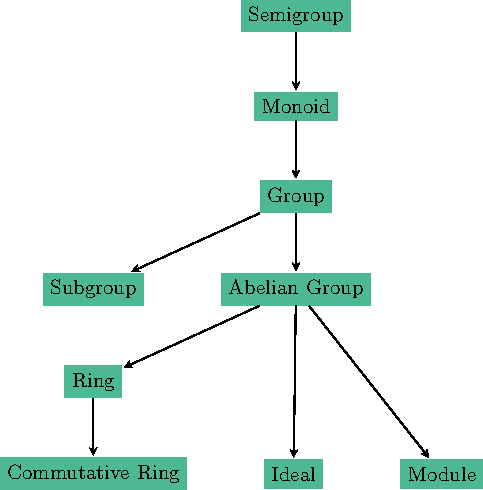
\includegraphics[width=.4\textwidth]{algebraic-structures.pdf}
  \centering
\end{figure}

\paragraph{Semigroups.} Our foundation begins by defining a semigroup class, which declares a binary
operation to be associative. From here, we build up through monoids, which
introduce identities, to groups, which introduce inverses. Note the double
equals ``$==$'' appearing in these definitions is notation for an arbitrary
equivalence relation over the group's carrier set, which acts as equality.

\begin{minted}{coq}
  Infix "==" := equiv (at level 60, no associativity).
  Class Semigroup := {
    semigroup_assoc:
      forall (a b c: Carrier),
        a <o> b <o> c == a <o> (b <o> c);
  }.
  Class Monoid := {
    monoid_semigroup :> Semigroup equiv op;
    monoid_ident_l:
      forall (a: Carrier), ident <o> a == a;
    monoid_ident_r:
      forall (a: Carrier), a <o> ident == a;
  }.
  Class Group := {
    group_monoid :> Monoid equiv op ident;
    group_inv_l:
      forall (a: Carrier), inv a <o> a == ident;
    group_inv_r:
      forall (a: Carrier), a <o> inv a == ident;
  }.
\end{minted}
The lines such as  ``\verb|monoid_semigroup :> Semigroup equiv op;|'' simply coerce
the monoid typeclass into a semigroup.


\paragraph{Algebraic quotients.}
While in the end, our formal proof does not call upon quotients of
algebraic structures, alternative proofs of Nakamaya's Lemma take advantage of 
 the structures quotient rings and quotient modules.  As algebraic 
 quotient structures are also fundamental to commutative algebra,
it is work pointing out that we have formalized quotients of groups, rings, and modules 
  using typeclasses, which appear to work rather smoothly. 

An algebraic quotient is, roughly, the set of equivalence classes of an
algebraic structure with respect to an equivalence relation on its elements,
for which the set of equivalence classes inherit the same kind of algebraic
structure. 
As an example, consider the quotient of a group modulo a subgroup,
i.e., a subset of elements of the group that it itself a group using the same operations. 
Under this equivalence relation on the group, every element of the
subgroup must be in the same equivalence class as the identity. 
For instance, after taking the quotient of the ring of integers $\mathbb{Z}$ by the
subgroup $n \mathbb{Z}$ consisting of all multiples of an integer $n$, one obtains the
group of integers modulo $n$, often denoted $\mathbb{Z}/n\mathbb{Z}$.
In general, with \texttt{P}
the predicate for the subgroup, there are two ways to make an equivalence
relation from this description.

\begin{minted}{coq}
  Definition left_congru (a b: Carrier) :=
    P (inv a <o> b).
  Definition right_congru (a b: Carrier) :=
    P (a <o> inv b).
\end{minted}

When these two equivalence relations coincide, then we can prove that this common
 relation actually preserves the group structure. Subgroups of a group that satisfy 
this property are called \emph{normal subgroups}.

\begin{minted}{coq}
  Let normal_subgroup_congru_coincide :=
    forall (a b: Carrier),
      left_congru op inv P a b <->
      right_congru op inv P a b.

  Theorem quotient_normal_subgroup_group:
    normal_subgroup_congru_coincide ->
    Group (left_congru op inv P) op ident inv.
\end{minted}

The utility--and, as a consequence, the ubiquity--of quotients in commutative algebra 
motivates our choice to use equivalence relations to define the components of a group structure. If one
were to instead use the traditional Leibniz equality, it would be difficult to
identify a quotient group with another group. However, by  defining a group in
terms of an arbitrary equivalence relation, in our theory a quotient group is 
simply defined as a group, but under an equivalence relation that is not the
usual equality. Not much is lost in adopting this convention thanks to Coq's 
rewrite tactics for setoids--types equipped with an equivalence relation---can 
still be called
upon.

\paragraph{Rings and their ideals.}
Moving onward, rings form the next step in our algebraic hierarchy; a ring has
two binary operations: addition, which must be commutative, and multiplication,
which need not be commutative in general. In our formulation, rings must have a
multiplicative identity. Next, we formalized the definition of a commutative
ring, further requiring commutativity of multiplication. At this point, we
formalized the notion of an ideal of a commutative ring, a subgroup of the ring
under addition that satisfies the absorption property under multiplication,
i.e., \(r a\) sits in the ideal whenever \(a\) of the ideal, regardless of the choice of 
element \(r\) of the commutative ring. We also used this to formalize the
notion of a quotient ring $R/I$, where $I$ is an ideal of a commutative ring
$R$.

Next, we formalized the definition of a  prime ideal, and then 
moved on to do the same for the notion of a maximal ideal, a proper ideal 
that is maximal with respect to inclusion. Below is the definition in Coq,
which uses \texttt{P} as the predicate for the ideal.

\begin{minted}{coq}
  Definition maximal_ideal :=
    exists (r: Carrier), (not (P r) /\
      forall (Q: Carrier -> Prop)
          (Q_proper: Proper (equiv ==> iff) Q)
          (Q_ideal: Ideal add zero minus mul Q),
        (forall (r: Carrier), P r -> Q r) ->
        (forall (r: Carrier), Q r) \/
          (forall (r: Carrier), Q r -> P r)).
\end{minted}

\noindent Next, we were able to employ this definition of a maximal ideal
to formally define a local
ring, i.e., a commutative ring with a single maximal ideal.
 
\begin{minted}{coq}
  Definition local_ring :=
    exists (P: Carrier -> Prop)
        (P_proper: Proper (equiv ==> iff) P)
        (P_ideal: Ideal add zero minus mul P),
      maximal_ideal P /\
      (forall (Q: Carrier -> Prop)
          (Q_proper: Proper (equiv ==> iff) Q)
          (Q_ideal: Ideal add zero minus mul Q),
        maximal_ideal Q -> forall (r: Carrier), P r <-> Q r).
\end{minted}

%\emily[inline]{Emily:  Unfortunately, I think we need to update naming
%  conventions since in mathematics, ``vector'' is reserved for an element of a
%  vector space over a field, rather than an element of an arbitrary module.  So
%  this could cause confusion.  Similar with ``basis,'' which is especially
%  tricking since two different generating sets of a finitely generated module
%  can have different sizes, but all bases of a vector space have the same
%  cardinality, and an element of a module can typically be written as a scalar
%  combination in multiple ways, while bases are linearly independent.  I've
%  proposed a rewrite of the blue paragraph right above it.  Drew, can you
%  double check it for accuracy with respect to the code? 
%}
%\emily[inline]{We'll also need to update the code.  I think {\ttfamily vectors}
%  should be something like {\ttfamily scalar-combinations}, and
%  {\ttfamily basis} something like {\ttfamily generating-set}. 
%}


\paragraph{Modules over rings.}
At this point, we formalized the definition of a module over a commutative ring,
the commutative-algebraic generalization of the notion of a vector space over a
field. Nakayama's Lemma is a statement about finitely generated modules, and
hence we formalized the notion of a scalar combination of a finite
collection of elements, $u_1, \ldots, u_n$ a module $M$ over a commutative ring $R$, i.e.,
expressions of the form $r_1 u_1 + r_1 u_2 + \cdots + r_n u_n$, where each
$r_i$ is an element of $R$.

In our formalization of scalar combinations, we use  ``list'' to mean
length-parameterized lists; since we don't use the simpler kind of lists, there
are no name collisions. In our code, \texttt{M} is the type of module elements,
\texttt{R} is the type of ring elements, act as coefficients, and
\texttt{t A n} is a list whose elements are of type \texttt{A} and whose length
is \texttt{n}.

\begin{minted}{coq}
  Definition finitely_generated {n: nat}(generatingSet: t M n) :=
    forall (elt: M),
      exists (coeffs: t R n),
        elt =M= linear_combin coeffs generatingSet.
\end{minted}

Finally, we defined the submodule $IM$ of a module $M$ over a commutative ring $R$, 
where $I$ is an arbitrary ideal of $R$.
Recall that when $R$ is local and $I$ is its unique maximal ideal, this submodule 
appears in the statement of Nakayama's Lemma. 
In general, $IM$ is the set consisting of all scalar
combinations of elements of \(M\) whose coefficients are in  \(I\). We
represent this in Coq as a predicate over \(M\).

\begin{minted}{coq}
  Context (P: R -> Prop).
  Context {P_proper: Proper (Requiv ==> iff) P}.
  Context {P_ideal: Ideal Radd Rzero Rminus Rmul P}.
  
  Definition ideal_module (x: M): Prop :=
    exists (n: nat)(coeffs: t R n)(elts: t M n),
      Forall P coeffs /\
      x =M= linear_combin Madd Mzero action coeffs elts.
\end{minted}

\noindent The use of  ``\verb|Forall P coeffs|'' ensures that every element of the
coefficient list \texttt{coeffs} satisfies the predicate \texttt{P}.  

\subsection{Constructing the Formal Proof}
Beyond formalizing the relevant structures from higher algebra, we also
formally establish some basic theory. For instance, a \emph{unit} of a
commutative ring $R$ is an element $x \in R$ with a multiplicative inverse,
i.e., an element $x^{-1} \in R$ for which $x \cdot x^{-1}$ is the
multiplicative identity $1 \in R$.  In fact, it $x$ is a unit, it has a unique 
inverse. 
 
We formally prove that an ideal $I$ of a commutative ring $R$ that contains a
unit $x$, then $I$ must be the trivial ideal, i.e., the entire ring.  The
informal logic is as follows:  Due to the absorption property of $I$,  
$x \cdot x^{-1} = 1 \in I$.  Hence for every element $r$ of $R$,
$r = r \cdot 1$ is also in $I$, i.e., $I=R$. 

Every non-unit element of a commutative ring is contained in some maximal
ideal, a fact that relies on the Axiom of Choice. 

The following standard informal
proof calls upon Zorn's lemma, which is equivalent to the Axiom of Choice, and
says that given a partially ordered set $S$, if every chain in $S$ has an upper
bound, then $S$ must have at least one maximal element. 

\begin{quote}
    Set \(I_{1}\) to be the principal ideal generated by an element \(x\) of a
    commutative ring $R$, i.e. the smallest ideal containing the element $x$,
    which consists of all $R$-multiples of $x$.
   
    If \(I_{1}\) is not a maximal ideal, then there exists a strictly larger
    proper ideal \(I_{2}\) of $R$, i.e.,
    $x\in I_{1}\subsetneq I_{2} \subsetneq R$. Moreover, if  \(I_{2}\) is not
    maximal, then there exists a strictly larger proper ideal
    $I_{3}$ containing $I_2$.
    
    Continuing this process, if it terminates at some step, we have found a
    maximal ideal, and if not, one obtains an infinite chain of ideals
    containing \(x\).
    \[x\in I_{1}\subsetneq I_{2}\subsetneq I_{3}\subsetneq\cdots\subsetneq R\]
    
    It is straightforward to verify that the increasing union of all $I_{k}$,
    $k \geq 1$, is by definition an ideal of $R$, and certainly
    contains \(x\).  Hence by Zorn's lemma, since every ascending chain of
    ideals containing $x$ with respect to inclusion has its union as an upper
    bound, there exists a maximal ideal of \(R\) containing \(x\).
\end{quote}

The above argument has potentially infinitely many steps. A proof with infinitely
many steps is a problem in Coq. To see this from the above argument, suppose we
wrote a proof tactic \mintinline{coq}{generate_larger_ideal} that allows us to
go from one non-maximal ideal \(I_{k}\) which contains \(x\) to another ideal
\(I_{k+1}\) which also contains \(x\). Provided our first ideal \(I_{1}\) is
not maximal, our first invocation of \mintinline{coq}{generate_larger_ideal}
will produce another ideal \(I_{2}\). Our new ideal \(I_{2}\) may also not be
maximal, requiring that we invoke \mintinline{coq}{generate_larger_ideal}
again. This can lead to an infinite number of calls to the tactic
\mintinline{coq}{generate_larger_ideal} which will occupy any machine's
processor(s) forever, and further, the infinite number of ideals in the proof
state will fill any machine's memory. After we have overwhelmed any system with
these infinite number of calls to a single proof tactic, we still have to
invoke more tactics to finish the proof with an application of Zorn's lemma,
which finally guarantees us a maximal ideal containing \(x\). To summarize, we
are forced to run the following proof script which will never get past calling
\mintinline{coq}{generate_larger_ideal} infinitely many times.
\begin{minted}{coq}
  repeat generate_larger_ideal. (* must be called infinitely often *)
  zorns_lemma. (* called after the above non-terminating call finishes *)
\end{minted}
We chose to avoid this infinite proof script issue by including an axiom that
any non-unit \(x\) of a ring must be contained in some maximal ideal.

\begin{minted}{coq}
Axiom comm_ring_nonunit_maximal_ideal:
  forall (x: Carrier),
    ~ is_unit equiv mul one x ->
    exists (P: Carrier -> Prop)(P_proper: Proper (equiv ==> iff) P)
    	(P_ideal: Ideal add zero minus mul P),
      P x /\ maximal_ideal P.
\end{minted} 

We also used classical logic to prove that \(1 - x\) is a unit whenever \(x\)
is an element of a local ring that is not a unit. The proof is completed by way
of contradiction, and uses the rule that \(\neg\neg P\rightarrow P\).

To start describing our proof, we formalize the statement of Nakayama's Lemma
in Coq.

\begin{nak*}
Let $R$ be a commutative local ring, and let $\mathfrak{m}$ denote its maximal
ideal. Suppose that $M$ is a finitely generated $R$-module. If
$M = \mathfrak{m} M$, then $M = 0$, i.e., $M$ must be the $R$-module containing
only one element, its identity as an additive abelian group. 
\end{nak*}

\begin{minted}{coq}
Context {P_ideal: Ideal Radd Rzero Rminus Rmul P}.
Context {P_maxideal: maximal_ideal Requiv Radd Rzero Rminus Rmul P}.
Context {R_local: local_ring Requiv Radd Rzero Rminus Rmul}.
  
Let ideal_module_pred := ideal_module Mequiv Madd Mzero action P.

Theorem nakayama:
  forall {n: nat}(basis: t M n),
    finitely_generated Mequiv Madd Mzero action basis ->
  (forall a: M, ideal_module_pred a) ->
  forall a: M, a =M= Mzero.
\end{minted}

To use as a building block in the formal proof of Nakayama's Lemma, we first
formally stated and proved a lemma that gives a concrete description of the
elements of the submodule $\mathfrak{m} M$  appearing in the statement of the
theorem. This lemma applies more generally, to any finitely generated module
$M$ over a (not necessarily local) commutative ring, and any submodule of the
form $I M$, for $I$ an arbitrary ideal. By definition, $IM$ consists of scalar
combinations of elements of $M$ with coefficients in $I$. The lemma states that
the elements from $M$ appearing in the expression can be chosen to be from any
fixed finite generating set for $M$. In other words, given any generating set
$u_{1},\dots, u_{n} \in M$  of a  finitely generated $R$-module $M$, every
element $x$ of $I M$ can be written as a scalar combination $a_1 \cdot u_1 +
a_2  \cdot u_2 + \cdots + a_n  \cdot u_n$, where each $a_i \in I$. 

\begin{minted}{coq}
Lemma module_fin_gen_ideal_module:
  forall {n: nat}(generatingSet: t M n),
    finitely_generated Mequiv Madd Mzero action generatingSet ->
    forall {m: nat}(coeffs: t R m)(elts: t M m),
      Forall P coeffs ->
      exists (coeffs': t R n),
        linear_combin Madd Mzero action coeffs elts =M=
          linear_combin Madd Mzero action coeffs' generatingSet /\
        Forall P coeffs'.
\end{minted}        

The proof follows from a straightforward argument based on definitions, by
induction on the number of elements in a fixed generating set for $M$, which we
informally describe: By definition, $x \in I M$ can  be written, for some
positive integer $k$ and elements $r_i \in R$ and $w_i \in M$,
$1 \leq i \leq k$, as $x = r_1 \cdot w_1 + r_2 \cdot w_2 + \cdots +
r_k \cdot w_k$. What's more, by definition of a finite generating set $u_{1},
\dots, u_{n}$ for $M$, each $w_i$ equals $c_{i1} \cdot u_1 + c_{i2} \cdot u_2 +
\cdots + c_{in} \cdot u_n$ for appropriate choices of $c_{ij} \in R$. Hence,
inductively applying associativity, 
\begin{align*}
  x = \sum_{i=1}^{k} r_i \cdot w_i
    = \sum_{i=1}^{k} r_i \cdot \left(\sum_{j=1}^n c_{ij} \cdot  u_j\right)
    = \sum_{j=1}^{n}\sum_{i=1}^{k} r_i \cdot (c_{ij} \cdot u_j) 
    = \sum_{j=1}^{n}\left(\sum_{i=1}^{k} c_{ij} \cdot r_i\right) \cdot u_j.   
\end{align*}
By absorption in ideals, each  $c_{ij}  \cdot r_i$ is in $I$, and since ideals
are closed under addition, we inductively conclude that the coefficient $a_j
:= c_{1j} \cdot  r_1 +  c_{2j} \cdot  r_2 +  \cdots c_{kj}\cdot r_k$ of $u_j$
is also in $I$. 

Now we move forward to outline the formal proof of Nakayama's lemma. We proceed
by induction on the number of elements in a generating set for the $R$-module
$M$. The base case is the situation when \(M\) requires no generators, so $M$
consists solely of the empty scalar combination, i.e., the empty sum, which, by
convention, is the zero element. In other words, $M = 0$ by assumption, and
this is also precisely the conclusion of Nakayama's Lemma.  Hence the statement
trivially, without using the hypothesis that $M = \mathfrak{m} M$.

We turn to the inductive step.  Fixing an arbitrary nonnegative integer $n$, 
we assume that Nakayama's Lemma holds in the case that $M$ has a generating set 
consisting of $n$ elements. 

Now, fix an $R$-module $M$ generated by $u_1, \ldots, u_{n+1} \in M$. By
assumption, \(M = \mathfrak{m} M\), and in particular, the generator $u_1$ is
an element of the submodule $\mathfrak{m} M$. The lemma described above
guarantees the existence of ring elements $a_1, \ldots, a_n \in \mathfrak{m}$
for which 
\[u_{1} = a_{1} \cdot u_{1} + a_2 \cdot u_2 + \cdots + a_{n+1} \cdot u_{n+1}.\]

Collecting the \(u_{1}\) terms on the left-hand side of the equation, applying
the existence of additive inverses in $R$, and distributivity of scalar
multiplication for modules, we see that
\begin{equation}\label{equation1: e}
(1 - a_{1}) \cdot u_{1} =
  a_{2} \cdot u_{2} + \cdots + a_{n+1} \cdot u_{n+1}\text{.}
\end{equation}
In Coq, we worked backwards to establish this fact. The comments following
each tactic offers a brief explanation of the effects on the goal.
\begin{minted}[linenos,firstnumber=157,stepnumber=5]{coq}
  assert ((Rone [+] Rminus a1) <.> u1 =M= (* (1 - a1) u1 = ... *)
    linear_combin Madd Mzero action coeffs' generatingSet').
  { setoid_rewrite (module_distrib_Radd Radd Rmul Rone
      Mequiv Madd Mzero Mminus action). (* 1 u1 + (-a1) u1 = ... *)
    setoid_rewrite (module_Rone Radd Rmul Rone
      Mequiv Madd Mzero Mminus action). (* u1 + (-a1) u1 = ... *)
    setoid_rewrite (module_minus_l Requiv Radd Rzero Rminus Rmul Rone
      Mequiv Madd Mzero Mminus action). (* u1 - a1 u1 = ... *)
    symmetry. (* ... = u1 - a1 u1 *)
    apply (group_move_r Mequiv Madd Mzero Mminus). (* ... + a1 u1 = u1 *)
    symmetry. (* u1 = ... + a1 u1 *)
    assumption. }
\end{minted}

Since a proper ideal contains no units and $a_1$ is taken to be in
$\mathfrak{m}$, it is not a unit. Hence, by the formalized statement mentioned
earlier, $1 - a_{1}$ is a unit of $R$. Let $b_{1} \in R$ denote its 
multiplicative inverse, so that $b_1 \cdot  (1 - a_{1}) = 1$. Multiplying this
element on the either side of \eqref{equation1: e}, we deduce the following.  
\begin{align*}
b_1 \cdot \left((1 - a_{1}) \cdot u_{1} \right)
  & = b_1 \cdot (a_{2} \cdot u_{2} + \cdots + a_{n+1} \cdot u_{n+1}) \\
\left( b_1 \cdot (1 - a_{1})\right) \cdot u_{1}
  & = b_1 \cdot (a_{2} \cdot u_{2}) + \cdots + b_1 \cdot (a_{n+1} \cdot u_{n+1}) \\
u_1 = 1 \cdot u_{1}
  & = (b_1 \cdot  a_{2}) \cdot u_{2} + \cdots + (b_1  \cdot  a_{n+1}) \cdot u_{n+1}  
\end{align*}
\begin{minted}[linenos,firstnumber=181,stepnumber=5]{coq}
  pose proof
    (local_comm_ring_sub_1_nonunit Requiv Radd Rzero Rminus Rmul Rone
      R_local x1 Hx1_nonunit) as H1ma1_unit.
  (* Getting to u1 = (b1 coeffs') . generatingSet *)
  inversion_clear H1ma1_unit as [b1 Hb1]. (* 1 - a1 is a unit *)
  setoid_rewrite (commutative Requiv Rmul) in Hb1. (* b1 (1 - a1) = 1 *)
\end{minted}
This bit of proof code has the effect of naming \(b_{1}\) as the inverse of the
unit \(1 - a_{1}\) and storing in the hypothesis \texttt{Hb1} the equation
\(b_{1} (1 - a_{1}) = 1\). The remainder of the code goes on to multiply on the
left by \(b_{1}\) in the equation \texttt{H} in order to say that
\(b_{1} ((1 - a_{1}) u1) = b_{1} (a_{2} u_{2} + \cdots + a_{n+1} u_{n+1})\).
Going on to use the rules of module actions and hypothesis \texttt{Hb1}, we can
simplify the left hand side of \texttt{H} to be just \(u_{1}\).
\begin{minted}[linenos,firstnumber=last,stepnumber=5]{coq}
  apply (module_op_l Requiv Mequiv action) with (r:=b1) in H.
  setoid_rewrite <- (module_distrib_Rmul Radd Rmul Rone
    Mequiv Madd Mzero Mminus action) in H. (* H: (b1 (1 - a1)) u1 = ... *)
  setoid_rewrite Hb1 in H. (* H: (1) u1 = ... *)
  setoid_rewrite (module_Rone Radd Rmul Rone
    Mequiv Madd Mzero Mminus action) in H. (* H: u1 = ... *)
\end{minted}
In particular, the generator $u_1$ can be written as a scalar combination of
the $n$ generators $u_2, \ldots, u_{n+1}$, and is superfluous. Hence $M$ can be
generated by $n$ elements, and $M=0$ by the inductive hypothesis. 

\emily[inline]{Emily: Reflecting, I think it would be valuable to include at
least parts of the formal proof.  Pieces would work, though it is short, and it
could be ``broken up'' among the description of the informal argument.  As is,
our description of the proof focuses on the informal argument, which is not
``new''.}

Showing that the inductive hypothesis holds in Coq is more work than in this
informal proof, but this extra work is just a lot of bookkeeping.

\section{Conclusion}
TODO

\bibliographystyle{plain}
\bibliography{references}
\end{document}
